\chapter{Analýza}
Táto kapitola sa venuje analýze súčasnej webovej aplikácie, ktorá zahŕňa analýzu jej architektúry a databázového modelu. Následne sú vymedzené jednotlivé funkčné a nefunkčné požiadavky novej webovej aplikácie, na ktoré nadväzuje sekcia používateľských rolí. Záver kapitoly je určený pre analýzu prípadov použití, ktoré vyplývajú z funkčných požiadaviek.

\section{Analýza súčasnej aplikácie}
Táto sekcia sa zaoberá analýzou súčasnej aplikácie, ktorá bola vytvorená pre potreby neziskovej organizácie viesť evidenciu zvierat, vrhov, ich registrácií a ďaľších informácií.
Hlavným cieľom analýzy je zistenie súčasného riešenia aplikácie z pohľadu architektúry a štruktúry súčasnej databázy.

\subsection{Architektúra aplikácie}
Samotný kód aplikácie nie je členený -- skladá sa z jednej vrstvy -- čo znamená, že kód aplikácie zodpovedný za prístup do databázy, logiku aplikácie a zobrazenie aplikácie nie je od seba oddelený.

\begin{figure}[H]
\begin{minipage}[]{\linewidth}
\begin{minted}[xleftmargin=1.8em,linenos]{php}

<?php
...
get_header();
if (!is_user_logged_in()) { 
  echo ("<h1>Neautorizováno</h1>\n");
} else {
?>
<h1>Detail zvířete</h1>
<br>
<?php
  if (!empty($_REQUEST['id'])) {
    $req_id = $_REQUEST['id'];
    if (is_numeric($req_id)) {
      $sql_potkan = "SELECT * FROM `" . $tabulka_zvirata . "`
      WHERE `id_prvni_verze` = " . $req_id .
      " ORDER BY `id` DESC";
      $potkani = $wpdb->get_results(
      	$sql_potkan, ARRAY_A, 0
      );
      $zvire = $potkani[0];
      if ($zvire != null) {
?>
  <div id="zvire">
    <fieldset style="
    border: 1px solid #A0A0A0;
    margin: 2px;
    padding: 5px;">
      <legend style="padding: 5px;">
          Základní informace
      </legend>
      <span id="popis">Pohlaví:</span><span id="hodnota">
      <?php 
        if ($zvire['pohlavi'] == 'M') {
          echo ("kluk"); 
        }
        else if ($zvire['pohlavi'] == 'F') {
          echo ("holka"); 
        }
        else {
          echo ("????"); 
        }
      ?>
      </span><br>
      ...
    </fieldset>
  </div>
\end{minted}
\end{minipage}

\caption[Ukážka súboru vrhy\_detail\_zvirete.php]
{Ukážka súboru vrhy\_detail\_zvirete.php}
\label{current-code-example}
\end{figure}

Obrázok \ref{current-code-example} obsahuje ukážku súboru súčasnej aplikácie, ktorý je zodpovedný za zobrazenie detailov zvieraťa v danom vrhu. Z ukážky je možné postrehnúť vyššie spomenuté miešanie logiky zodpovednej za funkcionalitu aplikácie (riadok 1--6), kód zodpovedný za prístup do databázy (riadok 10--19) a v neposlednom rade logiku zobrazovania aplikácie (riadok 21--41).

Ako programovací jazyk súčasnej aplikácie bol použítý jazyk PHP, ktorý bol navrhnutý v roku 1994 Rasmusom Lerdorfom. Tento jazyk je univerzálny programovací jazyk na strane servera a je primárne určený na vývoj webových stránok \cite{co-je-php}.

Pre pridávanie, spracovanie a získavanie dát v aplikácii slúži open-source SQL databázový systém nazývaný MySQL, ktorý je vyvíjaný, distribuovaný a podporovaný spoločnosťou Oracle Corporation \cite{co-je-mysql}. 

\subsection{Databázový model aplikácie}\label{sucasny-model-db}
Neoddeliteľnou súčasťou tejto práce je analýza databázového modelu existujúcej aplikácie. Na základe tejto analýzy bude navrhnutá taká štruktúra databázy, ktorá nebude spôsobovať nekonzistentnosť a duplicitu dát v aplikácii.

Databáza súčasnej aplikácie sa skladá z nasledujúcich tabuliek: \\ \mintinline{php}{czkp_mimi}, \mintinline{php}{czkp_vrh}, \mintinline{php}{czkp_zvire}, \mintinline{php}{pp_informace}, \mintinline{php}{pp_miminka} a \mintinline{php}{pp_zadosti}.

\subsubsection{Popis tabuliek}
V tejto podsekcii sú popísané jednotlivé tabuľky, ich štruktúra a najmä význam stĺpcov, do ktorých sa jednotlivé dáta ukladajú.
Pre lepšiu predstavu štruktúry databázového modelu aplikácie sa v podsekcii \ref{schema-tabuliek} nachádza logický model databázy v grafickej podobe. 

Všetky tabuľky obsahujú umelo-vytvorený unikátny primárny kľúč záznamu zvaný \mintinline{php}{id}, podľa ktorého sa rozlišujú jednotlivé záznamy.

V nasledujúcich dvoch tabuľkách (\mintinline{php}{czkp_vrh} a \mintinline{php}{czkp_zvire}) sa vyskytujú tri rovnaké stĺpce, menovite \mintinline{php}{id_prvni_verze},  \mintinline{php}{datum_zaznamu} a  \mintinline{php}{uzivatel}. V stĺpci \mintinline{php}{id_prvni_verze} je uložený identifikátor (\mintinline{php}{id}) prvej verzie zvieraťa/vrhu. Stĺpec \mintinline{php}{datum_zaznamu} obsahuje dátum vytvorenia záznamu spolu s jeho časom a v stĺpci \mintinline{php}{uzivatel} sa nachádza identifikátor používateľa, ktorý daný záznam vytvoril. Tento identifikátor ukazuje na systémovú tabuľku \mintinline{php}{wp_users}, ktorá obsahuje informácie o používateľoch súčasného systému.

\subsubsection*{Tabuľka czkp\_vrh}

Táto tabuľka má za úlohu správu dát týkajúcich sa jednotlivých vrhov. Stĺpec \mintinline{php}{id_prvni_verze} odkazuje na prvý záznam daného vrhu. \\ V stĺpci \mintinline{php}{wp_id_majitel} je uložený identifikátor majiteľa vrhu ukazujúci na systémovú tabuľku \mintinline{php}{wp_users}. Stĺpce \mintinline{php}{otec} a \mintinline{php}{matka} slúžia k ukladaniu identifikátorov otca, resp. matky. Tento identifikátor pochádza z tabuľky \mintinline{php}{czkp_zvire}.

Následne sú do tejto tabuľky ukladané aj údaje ako označenie vrhu (v stĺpci \mintinline{php}{oznaceni}), typ vrhu (\mintinline{php}{typ_priznani}), línia vrhu (\mintinline{php}{linie}), gény vrhu \\ (\mintinline{php}{geny_vrhu}), jeho varietnosť (\mintinline{php}{varietnost}) či dátum narodenia \\ (\mintinline{php}{datum_narozeni}). U každého vrhu sa taktiež zaznamenáva chovná stanica (\mintinline{php}{chov_stanice}), v ktorej sa daný vrh narodil, prípadne kontakt na chovateľa, ktorý je uložený v stĺpci \mintinline{php}{chov_kontakt}. Dôležité informácie, ako počet narodených a odchovaných mláďať sa ukladajú do stĺpcov \mintinline{php}{nar_mladat}, prípadne \mintinline{php}{odchov_mladat}. Počet odchovaných mláďat sa delí na počet odchovaných samcov (\mintinline{php}{odch_kluci}) a samíc (\mintinline{php}{odch_holky}). Počet mláďat uvoľnených pre chov je možné nájsť v stĺpci \mintinline{php}{mlad_chovne}. Rozdiel odchovaných mláďat a mláďat uvoľnených pre chov sa rovná počtu mláďat určených na maznáčika --- tento údaj je možné nájsť v stĺpci \mintinline{php}{mlad_pet}.

Jednotlivé vrhy môžu byť zaregistrované pod klubom ČKP --- tieto registrácie sa taktiež nachádzajú v tabuľke \mintinline{php}{czkp_vrh}. Pre účely registrácie vrhu slúžia stĺpce \mintinline{php}{datum_registrace}, v ktorom je uložený dátum registrácie, \\ \mintinline{php}{reg_cislo_vrhu}, ktorý obsahuje registračné číslo vrhu a \mintinline{php}{rok_reg}, ktorý značí, v ktorom roku bol vrh zaregistrovaný. Registrátor, ktorý zaregistroval daný vrh, môže pripojiť poznámku počas registrácie vrhu, ktorá je uložená v stĺpci \mintinline{php}{poznamka_reg}.

Chovateľ daného vrhu môže taktiež vytvoriť poznámku k vrhu --- táto poznámka sa následne uloží do stĺpca \mintinline{php}{poznamka_chov}.

Ako posledný stĺpec nachádzajúci sa v tabuľke \mintinline{php}{czkp_vrh} je stĺpec \mintinline{php}{kompletni}, ktorý značí, či o uloženom vrhu sú dostupné kompletné informácie, avšak tento údaj sa v aplikácii nepoužíva.

\subsubsection*{Tabuľka czkp\_zvire}

Tabuľka \mintinline{php}{czkp_zvire} slúži na ukladanie informácií o jednotlivých zvieratách, ktoré sú sledované organizáciou.

Skladá sa zo stĺpca \mintinline{php}{id_prvni_verze}, ktorý odkazuje na prvý záznam daného zvieraťa v rovnakej tabuľke -- čo znamená, že pomocou tohto stĺpca sa dajú zistiť všetky úpravy daného vrhu spustením príslušného SQL príkazu.
Jej obsahom je taktiež stĺpec \mintinline{php}{datum_zaznamu}, ktorý je nastavený na dátum a čas vloženia záznamu do tabuľky. Stĺpec \mintinline{php}{uzivatel} obsahuje identifikátor používateľa, ktorý daný záznam vytvoril. Následne sa v tabuľke nachádzajú stĺpce \mintinline{php}{uzamceny_upravy}, \mintinline{php}{uzamceny_kdy} a \mintinline{php}{uzamceni_kdo}, ktoré sa ale v súčasnej aplikácii nevyužívali. Pri zvierati je potrebné ukladať jeho pohlavie -- to je uložené v stĺpci \mintinline{php}{pohlavi}. Dátum narodenia zvieraťa sa nachádza v stĺpci \mintinline{php}{datum_narozeni}.

Informácie o chovateľovi, resp. majiteľovi zvieraťa sa ukladajú do šiestich stĺpcov (3 a 3). V stĺpci \mintinline{php}{chovatel_ckp_id} je uložený identifikátor chovatela (z tabuľky \mintinline{php}{wp_users}), v \mintinline{php}{chovatel} meno chovateľa a v \mintinline{php}{chov_stanice} chovateľská stanica. Informácie o majiteľovi majú podobnú štruktúru, s tým rozdielom že sa dáta ukladajú do stĺpcov \mintinline{php}{majitel_ckp_id}, \mintinline{php}{majitel} a \mintinline{php}{majet_stanice}. V prípade, že chovateľ resp. majiteľ nepochádza z organizácie, jeho identifikátor zostáva prázdny.

Vonkajšie črty zvieraťa, ako farba očí, typ uší, typ srsti, znaky a farba srsti sa ukladajú do stĺpcov \mintinline{php}{barva_oci}, \mintinline{php}{typ_ucha}, \mintinline{php}{typ_srsti}, \mintinline{php}{bila_kresba} \\ a \mintinline{php}{barva_srsti}.
Pre ukladanie otca a matky zvieraťa slúžia stĺpce \mintinline{php}{matka} a \mintinline{php}{otec}, v ktorých sa nachádza jedinečný identifikátor nachádzajúci sa v tejto tabuľke. Pre účely zaznamenania, z akého vrhu dané zviera pochádza, slúži stĺpec \mintinline{php}{cis_vrhu}, ktoré obsahuje registračné číslo vrhu, z ktorého dané zviera pochádza. Avšak pre jednoznačnú identifkáciu vrhu, odkiaľ zviera pochádza, mal slúžiť stĺpec \mintinline{php}{id_ckp_vrhu} --- ten sa ale nepoužíva.

Pre potreby organizácie sa do tejto tabuľky ukladajú údaje o registrácii zvieraťa ---  a to typ registrácie (stĺpec \mintinline{php}{reg_ckp_typ}), číslo registrácie\\ (\mintinline{php}{reg_ckp_cislo}) a rok registrácie (stĺpec \mintinline{php}{reg_ckp_rok}). Toto platí iba v prípade, že zviera je zaregistrované pod klubom ČKP. Ak je zviera zaregistrované pod iným klubom, tak sa jeho registračné číslo ukladá do stĺpca \mintinline{php}{reg_c_ostatni}. Navyše sa ukladá aj identifikátor registrátora, ktorý dané zviera zaregistroval pod klubom ČKP do stĺpca \mintinline{php}{registrator}. V neposlednom rade je nutné ukladať aj dátum registrácie zvieraťa --- pre túto informáciu slúži stĺpec \mintinline{php}{datum_registrace}.

Informácie o dátume úmrtia a dôvodu úmrtia zvieraťa sa ukladajú do stĺpcov \mintinline{php}{datum_umrti}, resp. do stĺpca \mintinline{php}{duvod_umrti}.

Chovateľ zvieraťa si taktiež môže pridať poznámku k zvieraťu, ktorá je následne uložená v stĺpci \mintinline{php}{poznamka_chovatel}.

Medzi ďalšie informácie, ktoré sa zbierajú o zvierati, patrí aj informácia ohľadom rizikovosti chovu (stĺpec \mintinline{php}{rizikovost_chovu}) a prípadná poznámka, prečo je chov rizikový. Táto poznámka sa ukladá samostatne do stĺpca \mintinline{php}{riziko_pozn}.

Predposledný stĺpec \mintinline{php}{overeno_pk} obsahuje informáciu, či zviera bolo overené podľa plemennej knihy a stĺpec \mintinline{php}{pozn_edit} obsahuje poznámku, ktorá mohla byť vytvorená pri editácii zvieraťa.

\subsubsection*{Tabuľka czkp\_mimi}

Úlohou tejto tabuľky je ukladať informácie o mláďatách narodených v jednotlivých vrhoch.
Rozdiel medzi tabuľkou \mintinline{php}{czkp_mimi} a \mintinline{php}{czkp_zvire} spočíva v tom, že narozdiel od tabuľky \mintinline{php}{czkp_zvire}, v tejto tabuľke sú uložené iba mláďata, ktoré pochádzajú zo známeho vrhu.

Tabuľka obsahuje stĺpec \mintinline{php}{id_vrhu}, v ktorom je uložený identifikátor záznamu z tabuľky \mintinline{php}{czkp_vrh}. Podľa tohto stĺpcu vieme určiť, v akom vrhu sa dané mláďa narodilo. Pre ukladanie mena a pohlavia mláďata slúžia stĺpce \mintinline{php}{jmeno}, resp. \mintinline{php}{pohlavi}. Chovnosť mláďata sa ukladá do stĺpca \mintinline{php}{chov}. Stĺpec \mintinline{php}{chov_omez} ďalej slovne špecifikuje chovné obmedzenie mláďata. Pre organizáciu je potrebné sledovať, kto dané mláďa chová, a pre tento účel slúži stĺpec \mintinline{php}{chov_kdo}. Pre uloženie dodatočných informácií ohľadom mláďata, ako napríklad typ uší, typ srsti, farba srsti, farba očí a znaky slúžia stĺpce \mintinline{php}{typ_ucha}, \mintinline{php}{typ_srsti}, \mintinline{php}{barva_srsti}, \mintinline{php}{barva_oci} a \mintinline{php}{znaky}.

\subsubsection*{Tabuľka pp\_informace}

Do nasledujúcej tabuľky --- \mintinline{php}{pp_informace} --- sa ukladajú informácie spojené s jednotlivými vrhmi. Táto tabuľka nemá žiadnu spojitosť s tabuľkou \mintinline{php}{czkp_vrh}. Dôvod vzniku tejto tabuľky bol vývoj nadstavby nad pôvodnou aplikáciou.

Táto tabuľka obsahuje stĺpec \mintinline{php}{uzivatel}, ktorý obsahuje identifikátor majiteľa vrhu ukazujúci do tabuľky \mintinline{php}{wp_users}. Následne sa do tabuľky ukladajú údaje o samotnom vrhu, ako napríklad typ vrhu (\mintinline{php}{typ_vrhu}), jeho označenie (\mintinline{php}{vrh_oznaceni}), dátum narodenia (\mintinline{php}{vrh_narozeni}), varietnosť \\(\mintinline{php}{vrh_varietnost}), počet narodených a odchovaných mláďat (\mintinline{php}{vrh_nar_mladat}/\mintinline{php}{vrh_odch_mladat}) a počet odchovaných samcov a samíc (\mintinline{php}{vrh_odch_kluci}/\mintinline{php}{vrh_odch_holky}).

Každý vrh má matku a otca vrhu --- tieto údaje sú ukladané do stĺpcov \mintinline{php}{vrh_id_matka} a \mintinline{php}{vrh_id_otec}. Ich obsahom sú identifikátory rodičov daného vrhu. Títo rodičia pochádzajú z tabuľky \mintinline{php}{czkp_zvire}.

Informácie o chovateľovi vrhu sa ukladajú do dvoch stĺpcov, a to \mintinline{php}{chovatel} a \mintinline{php}{chov_kontakt}. Prvý z menovaných stĺpcov obsahuje meno chovateľa a druhý jeho kontakt.

Nakoľko každý vrh môže byť zaregistrovaný, je nutné ukladať údaje o ich registrácii. Pre tieto účely slúžia stĺpce  \mintinline{php}{reg_dat_vyplneni}, ktorý značí dátum požiadania o registráciu majiteľom vrhu, \mintinline{php}{reg_dat_schvaleni}, ktorý obsahuje dátum schválenia vrhu a \mintinline{php}{reg_cislo_vrhu} obsahujúci registračné číslo vrhu.

\subsubsection*{Tabuľka pp\_miminka}

Obsahom tabuľky \mintinline{php}{pp_miminka} sú mláďatá, ktoré boli narodené vo vrhoch uložených v predchádzajúcej tabuľke.

Aby bolo možné zistiť, ku ktorému vrhu jednotlivé mláďa patrí, bolo potrebné, aby tabuľka obsahovala stĺpec \mintinline{php}{id_pp}, ktorý obsahuje identifikátor vrhu, v ktorom sa mláďa narodilo. Tento identifikátor ukazuje do predchádzajúcej tabuľky,  \mintinline{php}{pp_informace}. Následne sa do tabuľky ukladajú dáta týkajúce sa predovšetkým samotného mláďata, ako napríklad jeho meno (\mintinline{php}{mimi_jmeno}), pohlavie (\mintinline{php}{mimi_pohlavi}), typ uší (\mintinline{php}{mimi_typ_ucha}), typ srsti (\mintinline{php}{mimi_typ_srsti}), farba srsti (\mintinline{php}{mimi_barva_srsti}), či farba očí (\mintinline{php}{mimi_barva_oci}) a jeho znaky (\mintinline{php}{mimi_znaky}). K danému zvieraťu taktiež prislúcha majiteľ, ktorý sa ukladá do stĺpca \mintinline{php}{mimi_majitel}. Okrem mena majiteľa sa ukladá nie len jeho kontakt (\mintinline{php}{mimi_maj_kontakt}), ale aj číslo preukazu majiteľa, v prípade že je zároveň členom organizácie (\mintinline{php}{mimi_maj_prukaz}). Medzi posledné informácie ukladajúce sa k danému mláďatu patrí taktiež informácia, či je mláďa určené pre chov (\mintinline{php}{mimi_chov}), prípadne chovné obmedzenie (\mintinline{php}{mimi_chov_omezeni}).

\subsubsection*{Tabuľka pp\_zadosti}

Posledná tabuľka, ktorá sa nachádza v databáze súčasnej aplikácie, je tabuľka s názvom \mintinline{php}{pp_zadosti}.
Táto tabuľka má za úlohu zhromažďovať dáta o poslaných, resp. (ne)schválených žiadostiach o schválenie vrhu. 
Narozdiel od predchádzajúcich tabuliek, v tejto tabuľke sa nachádzajú stĺpce obsahujúce informácie iba k daným žiadostiam.

Táto tabuľka obsahuje stĺpec \mintinline{php}{id_pp}, ktorého obsahom je identifikátor vrhu z tabuľky \mintinline{php}{pp_informace}, ktorého sa týka daná žiadosť o schválenie vrhu. Tabuľka následne obsahuje stĺpec \mintinline{php}{datum_odoslani}, ktorý je automaticky nastavený na dátum a čas odoslania žiadosti a \mintinline{php}{cas_odpovedi}, ktorý indikuje dátum a čas odpovedi registrátora na danú žiadosť.

Okrem týchto informácií sa v tabuľke nachádza informácia o type schvaľovaného vrhu (\mintinline{php}{typ_vrhu}), poznámka žiadateľa o schválenie vrhu \\ (\mintinline{php}{poznamka_chovatel}) a komentár registrátora ku žiadosti (\mintinline{php}{komentar}). V prípade, že je žiadosť schválená, \mintinline{php}{reg_cislo_vrhu} bude obsahovať registračné číslo vrhu a \mintinline{php}{rok_reg} rok registrácie daného vrhu.

\pagebreak 
\subsubsection{Databázová schéma}\label{schema-tabuliek}

V tejto podsekcii je možné nájsť logický model databázy v grafickej podobe, ktorý obsahuje schému tabuliek so vzťahmi medzi jednotlivými tabuľkami.

\begin{figure}[H]
	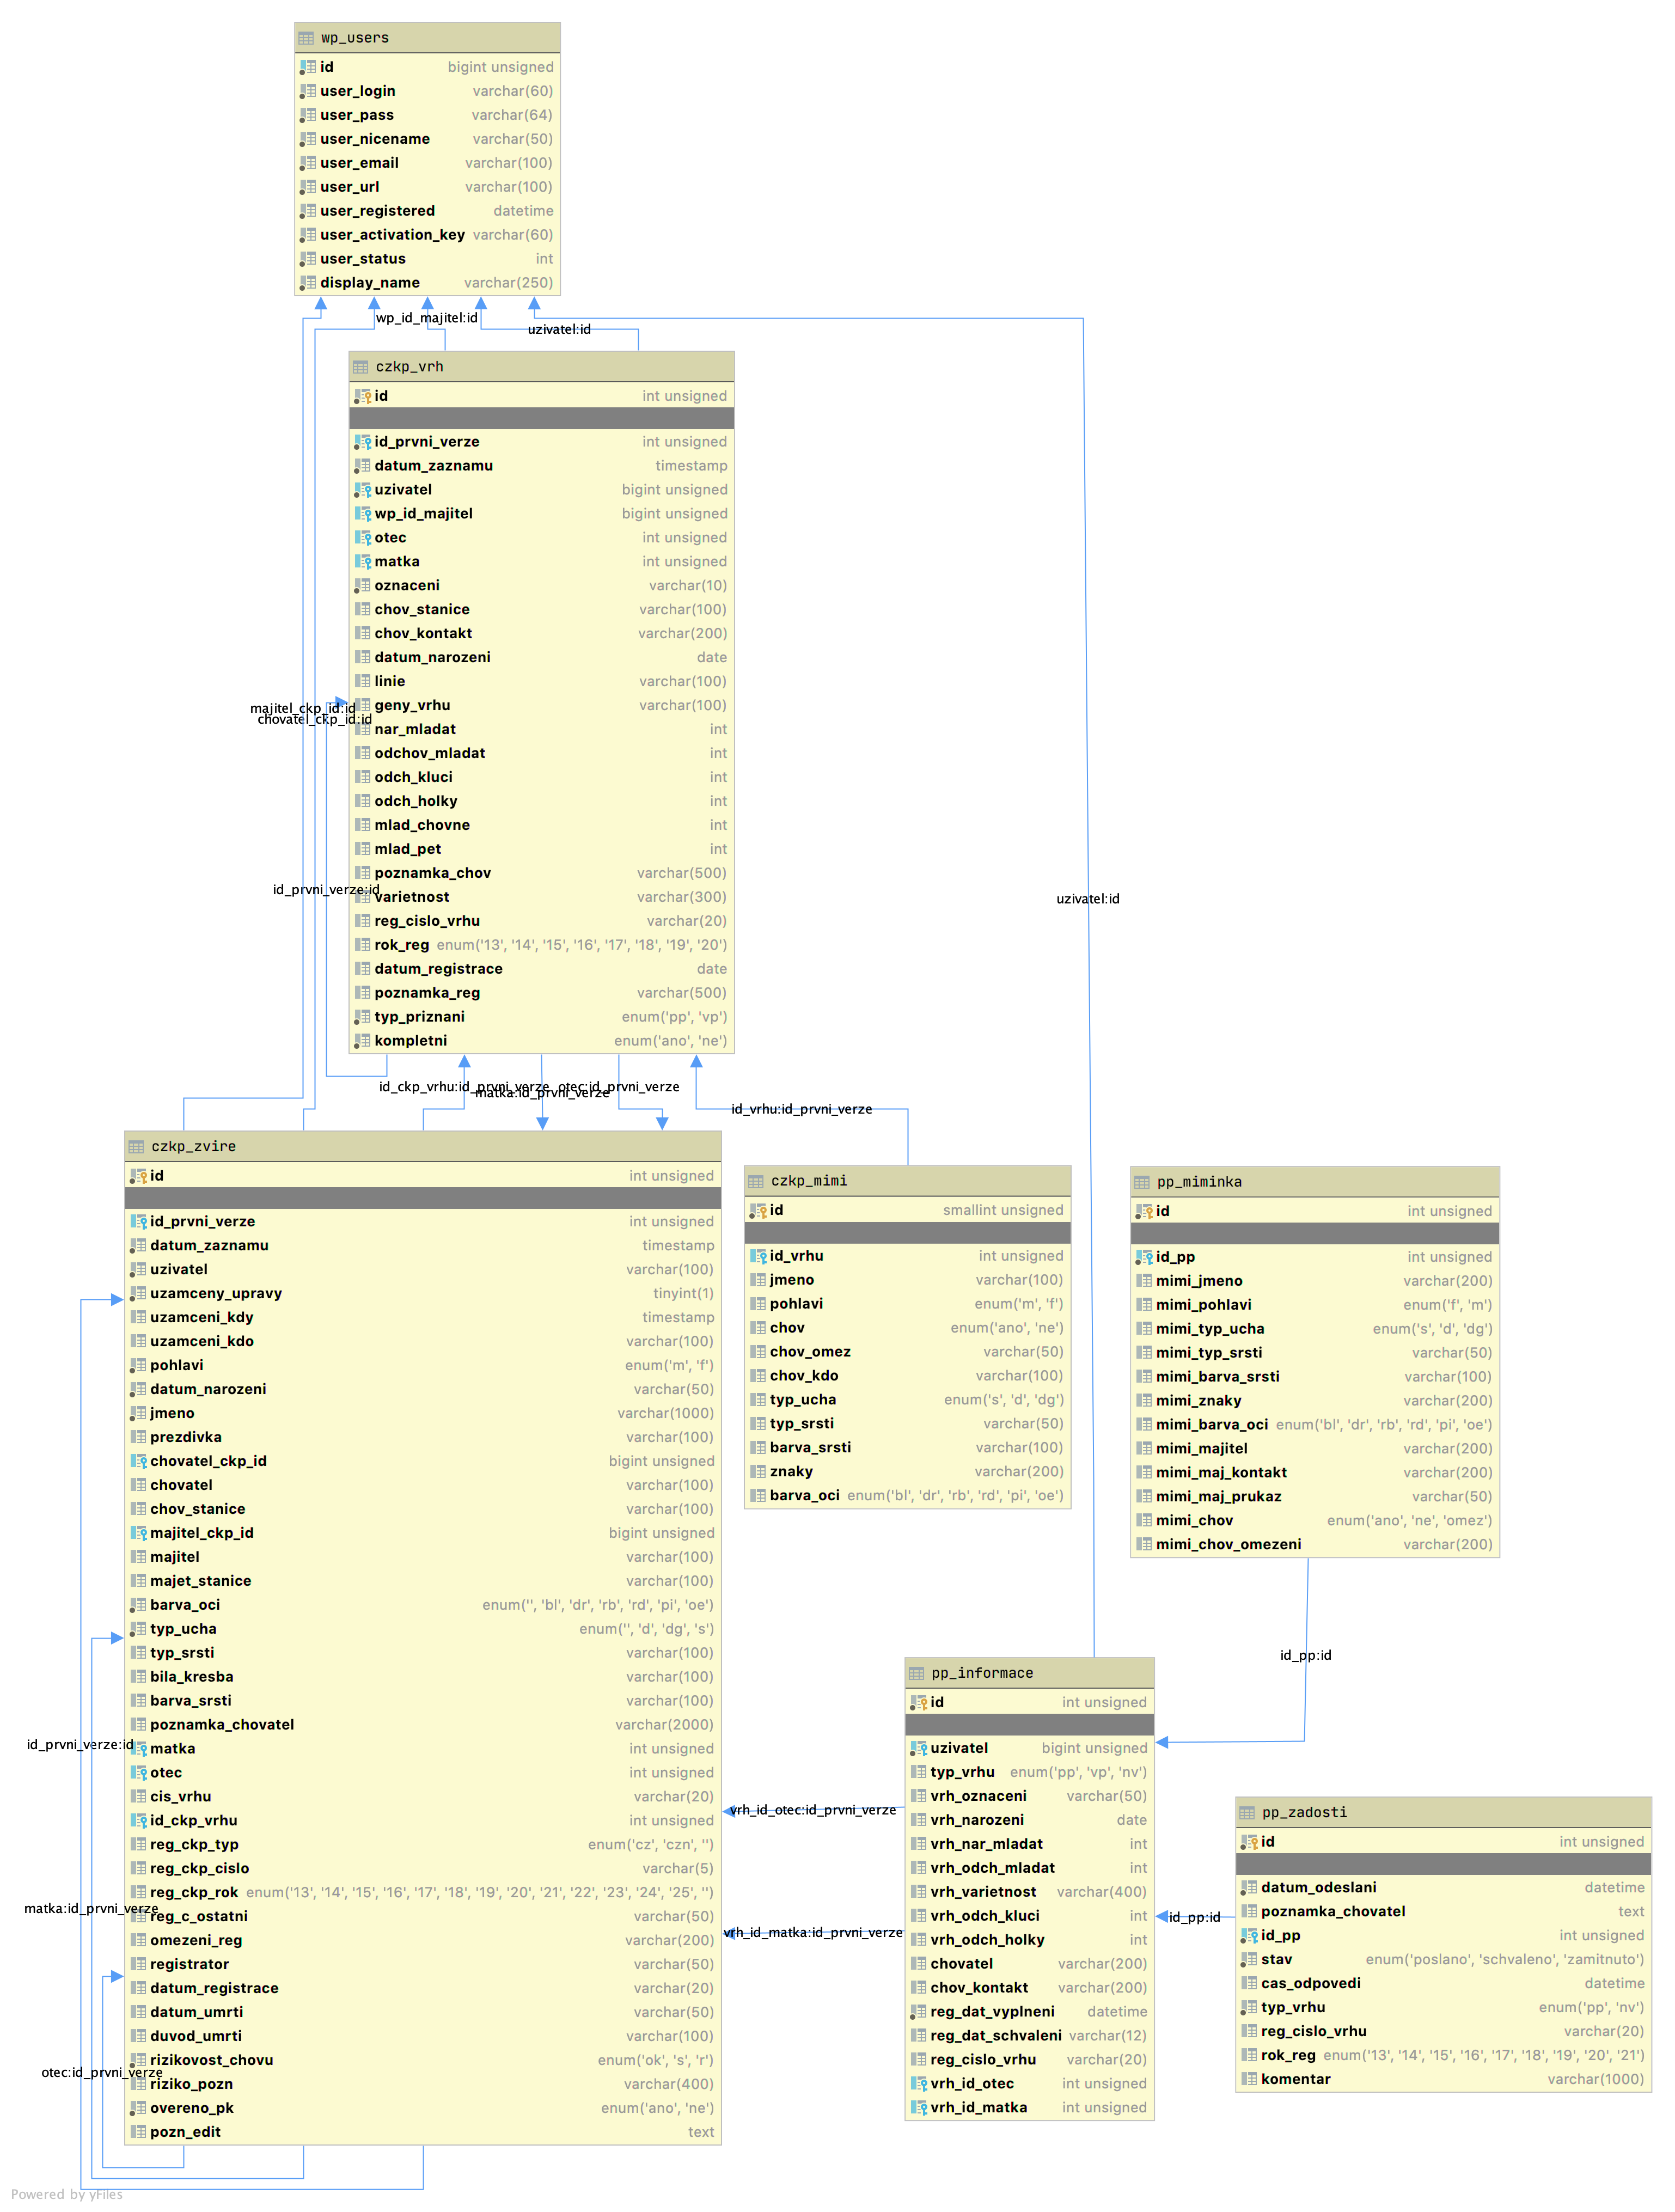
\includegraphics[width=1.0\textwidth]{media/analyza/diagram.png}
	\caption{Logický model databázy}
\end{figure}

\section{Analýza požiadaviek}
V tejto sekcii sa nachádza popis všetkých požiadaviek kladených na vznikajúcu webovú aplikáciu.
Tieto požiadavky delíme na funkčné a nefunkčné.

\subsection{Funkčné požiadavky}\label{funkcne-poziadavky}
Funkčné požiadavky vo všeobecnosti vymedzujú hranice aplikácie v kontexte jej funkcionality, ktorú používateľ od aplikácie očakáva. Ich úlohou je taktiež spresniť odhad pracnosti na vznikajúcej aplikácii \cite{funkcne-a-nefunkcne-poziadavky}.

\subsubsection{Evidencia zvierat}\label{evidencia-zvierat}
Aplikácia musí umožniť jednoduchú správu zvierat, od vytvorenia nového zvieraťa, cez zobrazenie jeho detailov, až po následnú editáciu, prípadne jeho zmazanie.

\hfill \break
V evidencii zvierat je pre každé zviera potrebné ukladať nasledujúce údaje:

\begin{itemize}
	\item meno a prezývku
	\item dátum narodenia
	\item majiteľa a chovateľa zvieraťa
	\item vrh, v ktorom sa zviera narodilo
	\item matku a otca zvieraťa
	\item pohlavie
	\item farbu očí
	\item typ uší
	\item farbu a typ srsti
	\item znaky
	\item dátum a dôvod úmrtia
\end{itemize}

Pre uľahčenie vytvorenia a editovania zvieraťa budú textové polia v maximálnej možnej miere interaktívne.

To znamená, že polia majiteľa a chovateľa zvieraťa vrátia na základe vstupu zoznam majiteľov, resp. chovateľov, ktorí už sú evidovaní v aplikácii. Následne si z tohto zoznamu používateľ zvolí požadovaného človeka.
V prípade, že aplikácia požadovaného človeka nevráti, používateľovi bude ponúknutá možnosť ho dodatočne vytvoriť.

Na podobnom princípe bude fungovať aj textové pole pre vrh, s tým rozdielom, že podľa zvoleného vrhu aplikácia predvyplní matku a otca zvieraťa.
 
\subsubsection{Evidencia registrácií zvieraťa}\label{evidencia-registracii-zvierata}
Je potrebné, aby aplikácia ponúkala možnosť zaregistrovať evidované zviera pod záujmový chov.
Pri takejto registrácií sa budú zbierať nasledovné údaje:

\begin{itemize}
	\item klub\footnote{Na výber z možností: ČKP, SOCHP alebo Ostatné}, pod ktorým bude zviera zaregistrované
	\item typ registrácie\footnote{Vyžadované iba v prípade registrácie zvieraťa pod klubom ČKP}
	\item registračné číslo
	\item dátum registrácie
	\item informácia, či je nasledovný chov povolený
	\item informácia o obmedzení chovu
\end{itemize}

\subsubsection{Evidencia vrhov}
Medzi nevyhnutnú funkcionalitu aplikácie sa radí aj evidencia vrhov. Tak ako pri evidencii zvierat, tak aj v tomto prípade používateľské rozhranie umožní vytvoriť nový vrh, zobraziť ho, respektíve ho editovať alebo vymazať. 

\hfill \break
Pre účel evidencie vrhov sa budú v aplikácii ukladať nasledujúce údaje:

\begin{itemize}
	\item typ a označenie vrhu
	\item majiteľ vrhu
	\item meno a kontakt na chovateľa
	\item dátum narodenia
	\item matka a otec vrhu
	\item línia
	\item genetické informácie
	\item počet narodených a odchovaných mláďat
	\item počet odchovaných samcov a samíc
	\item počet mláďat určených pre maznanie a pre následný chov
\end{itemize}

Rovnako ako pri evidencii zvierat, tak aj tu umožní aplikácia interaktívne zvoliť matku, otca a majiteľa vrhu zobrazením zoznamu uložených zvierat/ľudí.

\subsubsection{Správa žiadostí o schválenie vrhov}\label{sprava-ziadosti-o-schvalenie-vrhu}
Pre organizáciu je žiaduce, aby aplikácia obsahovala správu žiadostí o schválenie vrhu.

V rámci žiadosti o schválenie vrhu rozlišujeme dva typy osôb -- žiadateľa o schválenie vrhu\footnote{Zväčša majiteľ daného vrhu} a registrátora vrhu.

Aplikácia žiadateľovi umožní poslať žiadosť o schválenie vrhu s možnosťou zanechania poznámky pre registrátora.
Po odoslaní a úspešnom spracovaní tejto žiadosti serverom sa odošle e-mail všetkým registrátorom s informáciou o vytvorení novej žiadosti o schválenie vrhu. Na tento e-mail bude môcť zareagovať akýkoľvek registrátor, ktorý sa na základe dostupných informácií o vrhu rozhodne, či danú žiadosť schváli alebo zamietne.
O zmene stavu žiadosti bude žiadateľ informovaný e-mailom.

\subsubsection{Zobrazenie rodokmeňu zvieraťa a vrhu}\label{rodokmene}
Pre jednoduchšiu vizualizáciu predkov konkrétneho zvieraťa aplikácia ponúkne zobrazenie rodokmeňu zvieraťa vo forme jednoduchej tabuľky.

V tejto tabuľke budú okrem mien zvierat zobrazené aj dodatočné informácie o zvierati, definované v sekcii \ref{evidencia-zvierat}. Rodokmeň bude zobrazený v rámci jednotlivých zvierat a vrhov.

V prípade vrhu bude rodokmeň zobrazovať predkov matky a otca daného vrhu.

\subsubsection{Tvorba poznámok pre zviera a vrh}
V rámci aplikácie bude potrebné implementovať poznámky, ktoré budú môcť byť priradené jednotlivým zvieratám a vrhom.
Takáto poznámka by mala mať nastaviteľnú viditelnosť\footnote{Poznámka môže byť buď verejná alebo súkromná} a typ\footnote{Typ poznámky je jeden z nasledujúcich: všeobecná, upozornenie alebo výstraha}.
Taktiež musí poskytnúť informáciu, kedy bola vytvorená, respektíve editovaná.


Nakoľko sa jedná o poznámky pre zviera a vrh, budú zobrazené u príslušných zvieratách, resp. vrhoch, ku ktorým sa vzťahujú.

\subsubsection{Zobrazenie histórie zmien zvierat a vrhov}
Medzi želanú funkcionalitu novej webovej aplikácie patrí sledovanie a následné zobrazenie histórie zmien pre všetky zvieratá a vrhy

Aplikácia bude zaznamenávať nasledujúce zmeny v systéme:
\begin{itemize}
	\item vytvorenie zvieraťa/vrhu
	\item úprava údajov zvieraťa/vrhu
	\item zmazanie zvieraťa/vrhu
	\item obnova\footnote{Obnoviť zviera/vrh bude môcť iba administrátor aplikácie} zmazaného zvieraťa/vrhu
\end{itemize}

Pri každej zmene popísanej vyššie je taktiež nutné ukladať, kto a kedy danú zmenu vykonal. V prípade úpravy údajov budú navyše zaznamenané tie údaje, ktoré boli zmenené používateľom. Túto históriu zmien bude možné vidieť vo forme tabuľky u každého zvieraťa, resp. vrhu.

\subsubsection{Generovanie preukazov}\label{generovanie-preukazov}
Pre potreby organizácie je nevyhnutné implementovať generovanie preukazov (osvedčení) vo forme PDF súboru. V tomto súbore bude prvá strana vyplnená informáciami o danom zvierati \ref{evidencia-zvierat}, vrátane jeho registrácie zo sekcie \ref{evidencia-registracii-zvierata}. V niektorých prípadoch bude taktiež zobrazená registrácia vrhu v ktorom sa zviera narodilo, ktorej obsah je definovaný v \ref{sprava-ziadosti-o-schvalenie-vrhu}. Druhá strana súboru bude vyplnená rodokmeňom zvieraťa (\ref{rodokmene}).

Preukaz bude možné vygenerovať tlačidlom na stránke konkrétneho zvieraťa.

\subsubsection{Filtrovanie a radenie}\label{filtrovanie-a-radenie}
Pre vylepšenie používateľskej skúsenosti s aplikáciou bude potrebné implementovať filtrovanie a radenie zvierat ako aj vrhov na príslušných stránkach so zoznamom zvierat, resp. vrhov. Implementácia tejto funkcionality umožní jednoduchšiu prácu s aplikáciou a rýchlejšie nájdenie potrebných informácií.

\subsubsection{Správa používatelov a rolí}\label{sprava-pouzivatelov-a-roli}
Pre administrátorov aplikácie je nutné implementovať možnosť správy jednotlivých používateľov aplikácie, priradovať im príslušné role, alebo im ich naopak odoberať. Na základe tejto skutočnosti je žiaduce vytvoriť pohľad so zoznamom používateľov a ich rolami, s následnou možnosťou im danú rolu zmeniť, prípadne daných používateľov odobrať.

\subsubsection{Lokalizácia aplikácie}
Nakoľko budú aplikáciu používať nie len českí ale aj zahraniční používatelia, je nutné, aby aplikácia poskytovala obsah lokalizovaný do anglického jazyka. Jazyk bude možné jednoducho zmeniť v menu na paneli webovej aplikácie.

\subsection{Nefunkčné požiadavky}
Na rozdiel od funkčných požiadaviek, nefunkčné požiadavky umožňujú určiť obmedzenia kladené na aplikáciu. V neposlednom rade majú taktiež zásadný dopad na návrh architektúry webovej aplikácie \cite{funkcne-a-nefunkcne-poziadavky}.

\subsubsection{Webová aplikácia}
Nakoľko je požadovaný systém navrhnutý ako webová aplikácia, bude potrebné, aby bola prístupná z internetu pomocou moderných webových prehliadačov.

\subsubsection{Používateľské rozhranie}
Webová aplikácia bude musieť obsahovať používateľské rozhranie, s ktorým budú môcť používatelia interagovať.
Prostredie bude naviac responzívne, čo uľahčí prípadný prístup do systému z mobilného prehliadača.

\subsubsection{Technológie}
Po konzultácii s vedúcim práce boli vymedzené nasledovné technológie, ktoré budú použité na strane servera.

Ako programovací jazyk bude použítý jazyk PHP vo verzii 7.3, hoci momentálne existuje novšia verzia jazyku -- 7.4 \cite{verzie-php}.
Dôvod výberu nižšej verzie jazyka je daný PHP podporou webhostingu\footnote{Server poskytujúci webovú aplikáciu používateľom na internete, v tomto prípade sa jedná o webhosting Endora -- www.endora.cz}, na ktorom bude aplikácia nasadená.

Pre ukladanie dát potrebných pre funkčnosť aplikácie a ich následné spracovávanie bude použitý rovnaký databázový systém, ako v súčasnej aplikácii -- MySQL. Tento databázový systém bude použitý vo verzii 5.6.

Táto verzia taktiež nie je najnovšou verziou (v skutočnosti bola prvýkrát vydaná v roku 2013, avšak je stále oficiálne podporovaná \cite{verzie-mysql}), opäť z dôvodu neexistujúcej podpory novšieho databázového systému webhostingom.

\pagebreak

\section{Používateľské role}\label{pouzivatelske-role}
Novovznikajúca webová aplikácia bude prístupná iba zaregistrovaným a prihláseným používateľom. Navyše, niektoré akcie budú obmedzené iba pre určitý okruh používateľov.

K tomu, aby sme umožnili prístup k niektorým akciám iba vybraným používateľom, bude potrebné do aplikácie implementovať používateľské role a práva. Následne bude aplikácia riadiť prístup používateľa k jednotlivým akciám na základe príslušnosti k vybranej roli.

V nasledujúcich podsekciách budú priblížené jednotlivé role a k nim príslušné práva, ktoré sa budú vyskytovať v aplikácii.

\subsection{Bežný používateľ}\label{bezny-pouzivatel}
Túto rolu bude mať každý používateľ automaticky po registrácii do webovej aplikácie. Bežný používateľ bude môcť v aplikácii: 

\begin{itemize}
	\item Vytvoriť a zobraziť svoje zvieratá
	\item Upraviť svoje zvieratá v prípade, že nie sú zaregistrované pod klubom ČKP
	\item Vytvoriť a upraviť registrácie svojich vlastných zvierat, ktoré nespadajú pod klub ČKP
	\item Zobraziť zoznam všetkých cudzích zvierat spolu s ich detailmi
	\item Vytvoriť a zobraziť vrhy, u ktorých je používateľ ich majiteľom
	\item Upraviť vrhy, ktorých je majiteľom, pokiaľ neboli tieto vrhy schválené žiadosťou
	\item Zobraziť všetky vrhy typu VP alebo schválené vrhy typu PP a NV spolu s ich detailmi
	\item Pridať poznámku k zvieratám a vrhom, ktoré vlastní
\end{itemize}

\subsection{Registrátor zvierat}\label{registrator-zvierat}
Registrátor zvierat je v hierarchii rolí postavený nad bežným používateľom. Tým pádom má všetky práva bežného používateľa a navyše nasledujúce práva:

\begin{itemize}
	\item Možnosť pridať poznámku k akýmkoľvek zvieratám
	\item Možnosť pridať, editovať a vymazať akúkoľvek registráciu u každého zvieraťa
\end{itemize} 

\subsection{Schvalovateľ vrhov}\label{schvalovatel-vrhov}
Schvalovateľ vrhov je taktiež postavený v hierarchii rolí nad bežným používateľom podobne ako registrátor zvierat, s tým rozdielom, že schvalovateľ vrhu môže v aplikácii:

\begin{itemize}
	\item Vidieť a odpovedať na žiadosti o schválenie vrhov
	\item Editovať akékoľvek zviera a vrh
	\item Pridať poznámky k akémukoľvek vrhu
	\item Vygenerovať preukaz zvieraťa
\end{itemize}

\subsection{Administrátor}\label{administrator}
Ako obvykle, pre administrátora neplatia žiadne reštrikcie, čo znamená, že bude mať prístup ku všetkej funkcionalite definovanej vo funkčných požiadavkách v sekcii \ref{funkcne-poziadavky}.

\section{Prípady použitia}\label{pripady-pouzitia}
Prípady použitia sú špecifikácie rôznych činností, ktoré môžu používatelia s aplikáciou vykonávať \cite{co-su-pripady-pouzitia}. Tieto prípady použitia budú zachytené vo forme scenáru a budú vychádzať nielen zo známych funkčných požiadaviek popísaných v sekcii \ref{funkcne-poziadavky}, ale aj z jednotlivých používateľských rolí, ktoré boli definované v sekcii \ref{pouzivatelske-role}.

V tejto práci som sa rozhodol venovať iba takým prípadom použitia, ktoré sú z môjho pohľadu pre čitateľa prínosnejšie. Tie som následne rozdelil podľa príslušnosti k jednotlivým prvkom aplikácie. Všetky nasledujúce prípady použitia predpokladajú, že používateľ bude v systéme prihlásený.

\hfill \break
Poznámka: Prvé štyri scenáre použitia sú aplikovateľné aj na vrhy, avšak z dôvodu neuvádzania duplicitných informácií nebudú ďalej rozvinuté v príslušnej podsekcii. Zároveň pri následnej aplikácii prvých štyroch scenárov na vrhy, sa výskyt slova \uv{zviera} automaticky nahrádza slovom \uv{vrh} v príslušnej podobe.

\subsection{Prípady použitia zvierat}
V tejto podsekcii budú popísané jednotlivé prípady použitia, ktoré sa týkajú zvierat.

\subsubsection*{UC1 -- Vyhľadanie zvieraťa}\label{uc1}

Vyhľadanie zvieraťa je jeden zo základných prípadov použitia, kedy používateľ chce vyhľadať dané zviera.

\subsubsection*{Scenár:}

\begin{enumerate}
	\item Používateľ zvolí možnosť \uv{Zvieratá} z navigačného menu aplikácie.
	\item Aplikácia následne zobrazí tabuľku so zvieratami a filtrom, na základe ktorého si používateľ môže nastaviť dodatočné kritéria filtrovania zvierat.
	\item Používateľ nastaví filter podľa kritérií hľadaného zvieraťa a klikne na tlačidlo \uv{Filtrovať}.
	\item Aplikácia zobrazí všetky zvieratá vyhovujúce zadaným kritériám.
\end{enumerate}

\subsubsection*{Alternatívny scenár:}

\begin{enumerate}
    \item [3.] Aplikácia zobrazí hľadané zviera už po načítaní tabuľky so zvieratami. V tomto prípade scenár vyhľadávania zvieraťa končí.
\end{enumerate}

Tento prípad použitia realizuje viaceré funkčné požiadavky na aplikáciu, konkrétne \hyperref[evidencia-zvierat]{evidenciu} a \hyperref[filtrovanie-a-radenie]{filtrovanie a radenie} zvierat.

\subsubsection*{UC2 -- Zobrazenie detailu zvieraťa}\label{uc2}

Tento prípad použitia popisuje zobrazenie detailu zvieraťa a zahŕňa prípad \nameref{uc1}.

\subsubsection*{Scenár:}

\begin{enumerate}
	\item \nameref{uc1}
	\item Používateľ klikne na meno zvieraťa, ktorého detail si želá vidieť.
	\item Aplikácia zobrazí detail zvieraťa.
\end{enumerate}

Popísaný prípad taktiež realizuje funkčnú požiadavku na aplikáciu, a to \hyperref[evidencia-zvierat]{evidenciu zvierat}.

\subsection*{UC3 -- Vytvorenie zvieraťa}

Medzi ďalší základný prípad použitia patrí pridanie zvieraťa používateľom do systému.
Pri vytváraní zvieraťa sa aplikuje dodatočné obmedzenie pre bežného používateľa, ktoré spočíva v nemožnosti zvolenia majiteľa iného ako je on sám (\ref{bezny-pouzivatel}).

\subsubsection*{Scenár:}

\begin{enumerate}
	\item Používateľ zvolí možnosť \uv{Zvieratá} z navigačného menu aplikácie, ktorá následne načíta stránku so zoznamom uložených zvierat.
	\item Následne používateľ klikne na tlačidlo \uv{Pridať zviera}.
	\item Aplikácia načíta novú stránku s formulárom pre vytvorenie nového zvieraťa.
	\item Používateľ vyplní formulár.
	\item Po vyplnení všetkých potrebných údajov pre vytvorenie zvieraťa aplikácia umožní odoslať formulár kliknutím na tlačidlo \uv{Uložiť}.
	\item Používateľ klikne na tlačidlo \uv{Uložiť}.
	\item Po úspešnom vytvorení zvieraťa na základe vložených údajov systém presmeruje používateľa na stránku so zoznamom uložených zvierat.
\end{enumerate}

Tento prípad použitia realizuje funkčnú požiadavku \hyperref[evidencia-zvierat]{evidencie zvierat}.

\subsection*{UC4 -- Úprava zvieraťa}

V tomto prípade sa používateľ aplikácie snaží upraviť existujúce zviera v systéme. Tento prípad použitia taktiež zahŕňa prípady 
\nameref{uc1} alebo \nameref{uc2}, v závislosti od spôsobu úpravy zvieraťa, ktorý si používateľ zvolí.

\subsubsection*{Scenár:}

\begin{enumerate}
	\item \nameref{uc1}
	\item Používateľ klikne na rozbalovacie menu u zvieraťa, ktoré chce editovať.
	\item Po tomto kroku aplikácia ponúkne možnosť editácie alebo zmazania zvieraťa.
	\item Používateľ zvolí možnosť editácie.
	\item Aplikácia následne presmeruje používateľa na stránku s editáciou zvieraťa, ktorá bude obsahovať formulár s predvyplnenými údajmi zvieraťa.
	\item Používateľ upraví údaje zvieraťa.
	\item Kliknutím na tlačidlo \uv{Odoslať} sa odošle vyplnený formulár na server.
	\item Po úspešnom spracovaní formuláru je používateľ presmerovaný na stránku s detailmi upravovaného zvieraťa.
\end{enumerate}

\subsubsection*{Alternatívny scenár:}

\begin{enumerate}
	\item \nameref{uc2}
	\item Používateľ klikne na tlačidlo \uv{Upraviť} na pravom postrannom paneli.
	\item Následne scenár pokračuje bodom 5 v pôvodnom scenári.
\end{enumerate}

Popísaný prípad použitia realizuje funkčnú požiadavku \hyperref[evidencia-zvierat]{evidencie zvieraťa}.

\subsection*{UC5 -- Vytvorenie registrácie zvieraťa}

Tento prípad použitia popisuje vytvorenie registrácie zvieraťa. Pri samotnom vytváraní novej registrácie sa aplikujú dodatočné obmedzenia pre bežného používateľa, tak ako je popísane v \ref{bezny-pouzivatel}.

Tento prípad použitia zahŕňa prípad \hyperref[uc2]{zobrazenia detailov zvieraťa}.

\subsubsection*{Scenár:}

\begin{enumerate}
	\item \nameref{uc2}
	\item Kliknutím na tlačidlo \uv{Pridať novú registráciu} aplikácia zobrazí registračný formulár v modálnom okne\footnote{Menšie okno aplikácie prekrývajúce jej hlavný obsah}.
	\item Používateľ vyplní potrebné polia.
	\item Po stlačení tlačidla \uv{Uložiť} sa vyplnený formulár odošle na server.
	\item Po úspešnom spracovaní formuláru serverom sa modálne okno zavrie.
\end{enumerate}

Tento prípad použitia realizuje funkčnú požiadavku kladenú na aplikáciu, konkrétne \hyperref[evidencia-registracii-zvierata]{evidenciu registrácií zvieraťa}.

\subsection{Prípady použitia vrhov}
Táto podsekcia popisuje jednotlivé prípady použitie, ktoré sa týkajú vrhov.

\subsection*{UC6 -- Vytvorenie žiadosti o schválenie vrhu}

Tento prípad použitia reálne zahŕňa prípad použitia \uv{zobrazenia detailov vrhu}, avšak pre neuvádzanie duplicitných informácii môže čitateľ vychádzať z prípadu použitia \hyperref[uc2]{zobrazenia detailov zvieraťa}. Scenáre sa v oboch prípadoch obsahovo nelíšia, tak ako bolo uvedené poznámke v sekcii \ref{pripady-pouzitia}.

Na tento prípad sa taktiež vzťahujú dodatočné obmedzenia pre bežného používateľa vyplývajúce z \ref{bezny-pouzivatel}.

\subsection*{Scenár:}

\begin{enumerate}
	\item \nameref{uc2}
	\item Používateľ klikne na tlačidlo \uv{Vytvoriť žiadosť}.
	\item Aplikácia následne zobrazí modálne okno s formulárom obsahujúcim textové pole slúžiace pre poznámku registrátorovi.
	\item Po stlačení tlačidla \uv{Uložiť} sa formulár odošle na server.
	\item Po úspešnom spracovaní formuláru serverom sa vytvorí nová žiadosť o schválenie vrhu.
	\item Modálne okno sa automaticky zavrie.
\end{enumerate}

Popísaný prípad použitia realizuje funkčnú požiadavku \hyperref[sprava-ziadosti-o-schvalenie-vrhu]{správy žiadostí o schválenie vrhu}.

\subsection*{UC7 -- Odpoveď na žiadosť o schválenie vrhu}

Tak ako v predchádzajúcom prípade, tento prípad použitia bude zahŕňať \uv{zobrazenie detailov vrhu}.

Pre tento prípad použitia sa vzťahujú dodatočné obmedzenia -- na žiadosť o schválenie vrhu bude môcť odpovedať používateľ majúci rolu \hyperref[schvalovatel-vrhov]{schvalovateľa žiadostí vrhov} alebo \hyperref[administrator]{administrátora}.

\pagebreak 
\subsection*{Scenár:}

\begin{enumerate}
	\item \nameref{uc2}
	\item Používateľ stlačí tlačidlo \uv{Odpovedať} pri príslušnej žiadosti o schválenie vrhu.
	\item Aplikácia zobrazí modálne okno s formulárom pre schválenie vrhu.
	\item Používateľ vyplní formulár a kliknutím na tlačidlo \uv{Uložiť} sa odošle na server.
	\item Server spracuje odoslaný formulár a ihneď odošle e-mail žiadatelovi o stave jeho žiadosti.
\end{enumerate}

\subsection*{Alternatívny scenár:}

\begin{enumerate}
	\item Používateľ klikne na link v e-maili, ktorý mu prišiel po odoslaní novej žiadosti o schválenie vrhu žiadateľom.
	\item Ako reakcia na kliknutie na link, operačný systém otvorí predvolený webový prehliadač s adresou vedúcou na detail vrhu.
	\item Následne scenár pokračuje bodom 2 v pôvodnom scenári.
\end{enumerate}

Tak ako v predchádzajúcom prípade použitia, aj v tomto prípade použitia je realizovaná funkčná požiadavka \hyperref[sprava-ziadosti-o-schvalenie-vrhu]{správy žiadostí o schválenie vrhu}.
	